\documentclass{article}

% Obtain the official NeurIPS 2026 style from the conference website.
\usepackage[preprint]{neurips_2026}
\usepackage[utf8]{inputenc}
\usepackage[T1]{fontenc}
\usepackage{booktabs}
\usepackage{amsmath}
\usepackage{amssymb}
\usepackage{graphicx}
\usepackage{hyperref}
\usepackage{url}
\usepackage{enumitem}

\title{Ghost Wave Security: Sheaf-Inspired Multipolar Recovery for Disposable Infrastructure}
\author{0syamunyamu1 \\ Independent Researcher}

\begin{document}
\maketitle

\begin{abstract}
Ghost Wave Security is a concept-and-feasibility framework for recovery diversity in disposable software infrastructure. The architecture separates a protected persistent core from replaceable execution shells, measures graph-level local-to-global inconsistency using a small cellular-sheaf-inspired diagnostic, and compares recovery policies over E8, D8, and random spherical candidate codebooks. The E8 root system is not presented as cryptography or a literal infrastructure symmetry. It is a fixed and auditable hypothesis about candidate diversity. The accompanying simulator removes strategy-specific core-breach probabilities and prevents the defender from observing the attacker’s hidden state. Results are generated automatically and must be interpreted only within the synthetic benchmark.
\end{abstract}

\section{Introduction}
A defensive workflow that repeatedly restores the same shell may unintentionally provide an adaptive adversary with a stable target model. Moving Target Defense introduces controlled variation into exposed system properties \cite{jajodia2011mtd}, while Zero Trust Architecture separates access decisions from implicit network location \cite{rose2020zero}. Ghost Wave Security studies a narrower problem: after a disposable shell appears compromised, should recovery return to a familiar baseline or preserve multiple structurally different paths back to operation?

The proposed architecture has four parts: a Persistent Core, Disposable Shells, a Sheaf-Inspired Coherence Monitor, and a Multipolar Recovery Engine. The primary claim is modest: recovery diversity can be made explicit, measured, and compared under controlled toy dynamics.

\section{Architecture}
The Persistent Core stores approved recovery manifests, evidence, and policy constraints behind interfaces that do not expose secret material to the disposable layer. The minimum safety boundary is
\begin{equation}
\text{AI proposal} \neq \text{production authorization}.
\end{equation}

Let $G=(V,E)$ be a service dependency graph. Each node carries a local state $x_i=[r_i,a_i,p_i]$ containing risk, anomaly, and privilege drift. A fixed edge projection $R$ defines a residual
\begin{equation}
(\delta x)_{ij}=Rx_i-Rx_j,
\end{equation}
and the gluing energy is the mean squared residual over edges. This construction is sheaf-inspired but does not implement persistent sheaf cohomology.

The Collapse Index combines compromise fraction $C_t$, normalized gluing inconsistency $G_t$, and an observed route-concentration estimate $R_t$:
\begin{equation}
\mathrm{CI}_t=0.50C_t+0.30G_t+0.20R_t.
\end{equation}
When the index crosses a threshold, the shell is replaced. Diversity-constrained strategies score candidate shells by distance from a noisy defender estimate, distance from the current shell, similarity to recently used shells, and operational-change cost.

\section{Benchmark Design}
The simulator compares static defense, single rollback, random E8 rotation, diversity-constrained E8 recovery, diversity-constrained D8 recovery, and diversity-constrained random spherical recovery. The hidden attacker adapts to the current shell. The defender sees only noisy operational pressure. Core breach is produced by one shared hazard function for all strategies and depends on compromise extent, critical-node exposure, persistence, and graph inconsistency.

Static defense receives zero recovery downtime but accumulates compromised-service exposure cost and an explicit synthetic penalty if the persistent core is breached. This prevents unrecovered compromise from appearing operationally free.

\section{Generated Results}
\begin{table}[h]
\centering
\caption{Synthetic benchmark results generated by the repository. Lower is better.}
% Auto-generated by ghost_wave.benchmark. Do not edit manually.
\begin{tabular}{lrrrr}
\toprule
Strategy & Shell compromise & Core breach & Total cost & Mean CI \\
\midrule
ghost_d8 & 0.319 & 0.358 & 105.8 & 0.316 \\
ghost_e8 & 0.332 & 0.367 & 108.4 & 0.317 \\
ghost_random & 0.334 & 0.350 & 107.3 & 0.318 \\
random_e8 & 0.284 & 0.325 & 112.0 & 0.348 \\
single_rollback & 0.300 & 0.275 & 156.3 & 0.428 \\
static & 0.974 & 0.933 & 155.7 & 0.689 \\
\bottomrule
\end{tabular}

\end{table}

\begin{figure}[h]
\centering
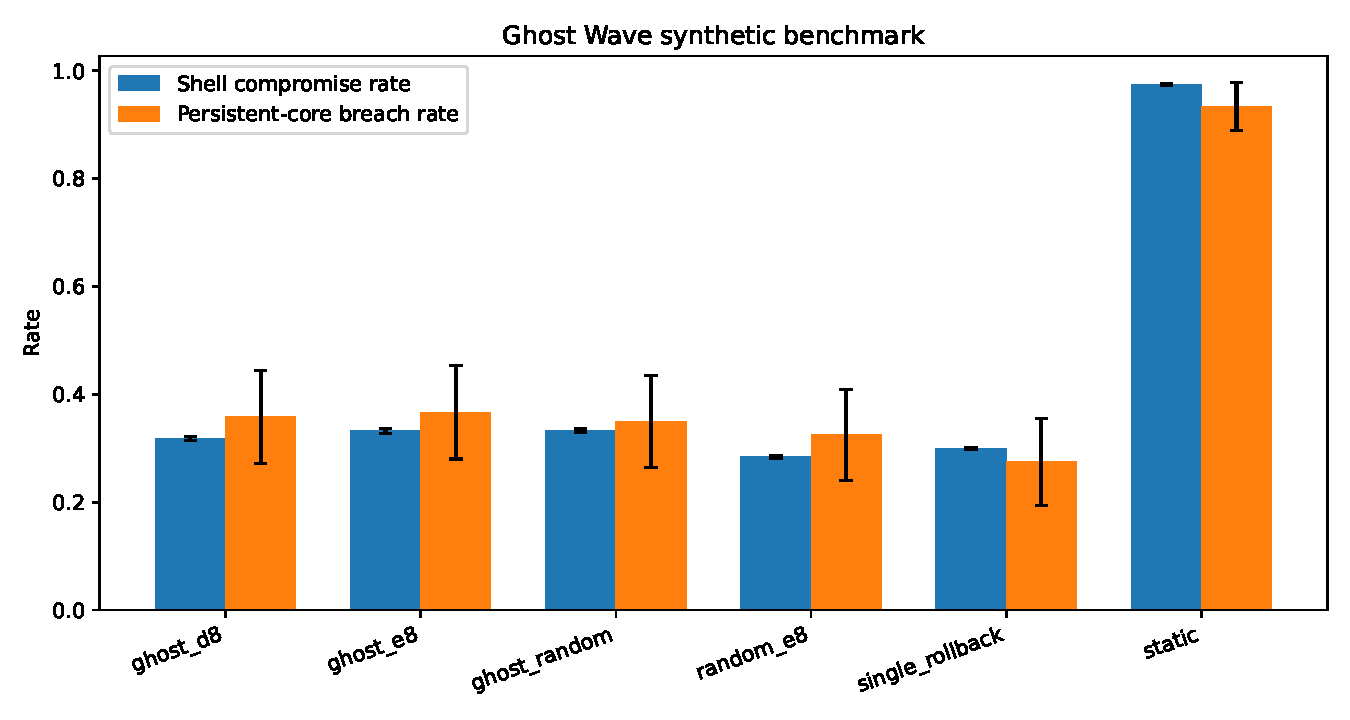
\includegraphics[width=0.95\linewidth]{../figures/benchmark_rates.pdf}
\caption{Synthetic shell-compromise and persistent-core breach rates with 95\% normal-approximation confidence intervals.}
\end{figure}

\section{Limitations and Safety Boundaries}
The benchmark does not model real vulnerabilities, production networks, or physical infrastructure. E8 may perform no better than D8 or random spherical candidates; the comparison is intended to expose this possibility. Automated recovery must remain rate-limited, logged, reversible, independently validated, and unable to access offline keys or external shutdown controls.

\section{Conclusion}
Ghost Wave Security asks systems to preserve what must not move, discard what can be replaced, and maintain more than one credible recovery direction. The present contribution is a reproducible test object, not a production security claim.

\bibliographystyle{plain}
\bibliography{references}
\end{document}
